\documentclass{beamer}
\usepackage{beamerthemeshadow}
\usepackage[utf8]{inputenc}  
\usepackage{longtable}
\usepackage[ngermanb]{babel}
\beamersetuncovermixins{\opaqueness<1>{25}}{\opaqueness<2->{15}}
\begin{document}

% Latex Beamer Übersicht: 
% https://www2.informatik.hu-berlin.de/~mischulz/beamer.html

\title{WebPiraten}  
\author{M. Rasch, A. Flohr, C. Nehls, M. Neumann}
\date{22.08.2014} 

\begin{frame}
\maketitle
\end{frame} 

\begin{frame}
\frametitle{Übersicht}
\tableofcontents
\end{frame}

\begin{frame}
\begin{itemize}
\item Demo
\item Übersichtgrafik
\item Use-Case (grob)\newline
-$>$ GUI -(websocket)-$>$ Preprocossor -(TCP)-$>$ VM -(STDIN)-$>$ Ausführung -(STDIN)-$>$ VM-Wrapper -(TCP)-$>$ Rails-Simulation -(websocket)-$>$ GUI $<$-
\item Preprocessor
\item VM
\item Simulation
\item Client
\item Erlang
\item Scopes
\item Sicherheit
\item Performance
\end{itemize}
\end{frame}

\subsection{Javascript-Client}

\begin{frame}
\begin{center}
	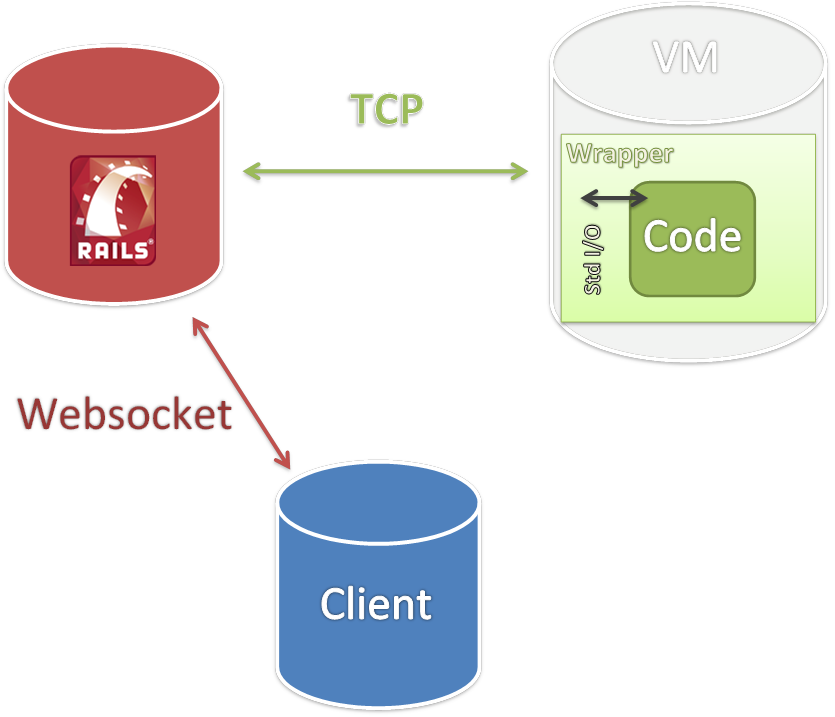
\includegraphics[scale=0.35]{overview}
\end{center}
\end{frame}

\begin{frame}
\frametitle{Web-Technologien}
\begin{center}
	
\includegraphics[scale=0.2]{client/HTML5_Logo.png}
	
\includegraphics[scale=0.2]{client/css3logo.png}
	
\end{center}		
	
	
	
\includegraphics[scale=0.4]{client/coffeescript-logo.png}
	
\includegraphics[scale=0.40]{client/less-logo.png}
	
\includegraphics[scale=0.045]{client/bootstrap-logo.png}
\end{frame}

\begin{frame}
\frametitle{Javascript-Client}
\begin{center}
	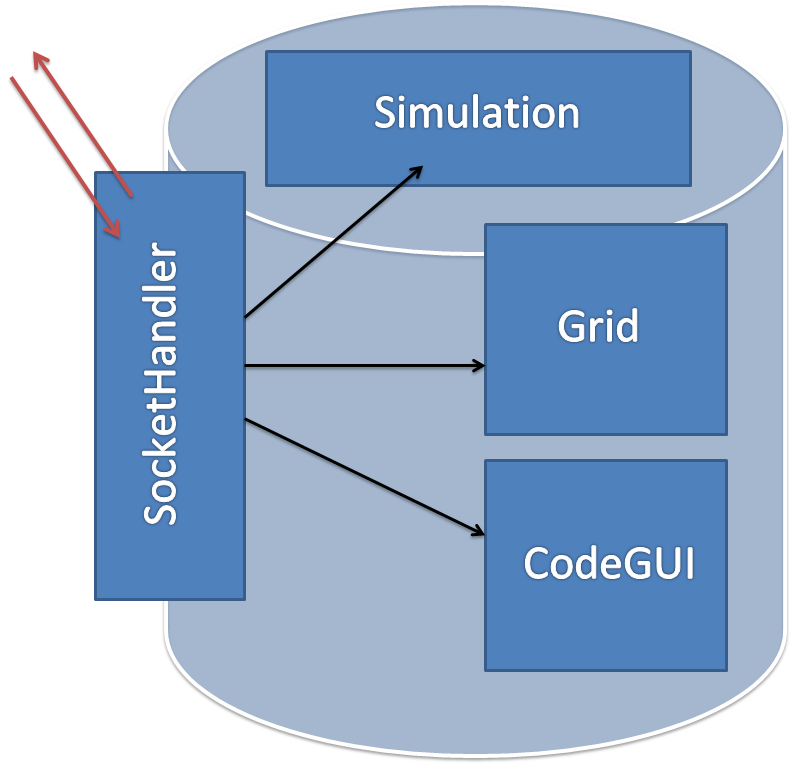
\includegraphics[scale=0.3]{client/modules.png}
\end{center}
\end{frame}


\begin{frame}
\frametitle{SocketHandler}
\inputminted[linenos, numbersep=2pt, tabsize=4, frame=lines, label=Beispiel Paket]{json}{client/packet.json}
\end{frame}

\begin{frame}
\frametitle{SocketHandler}
	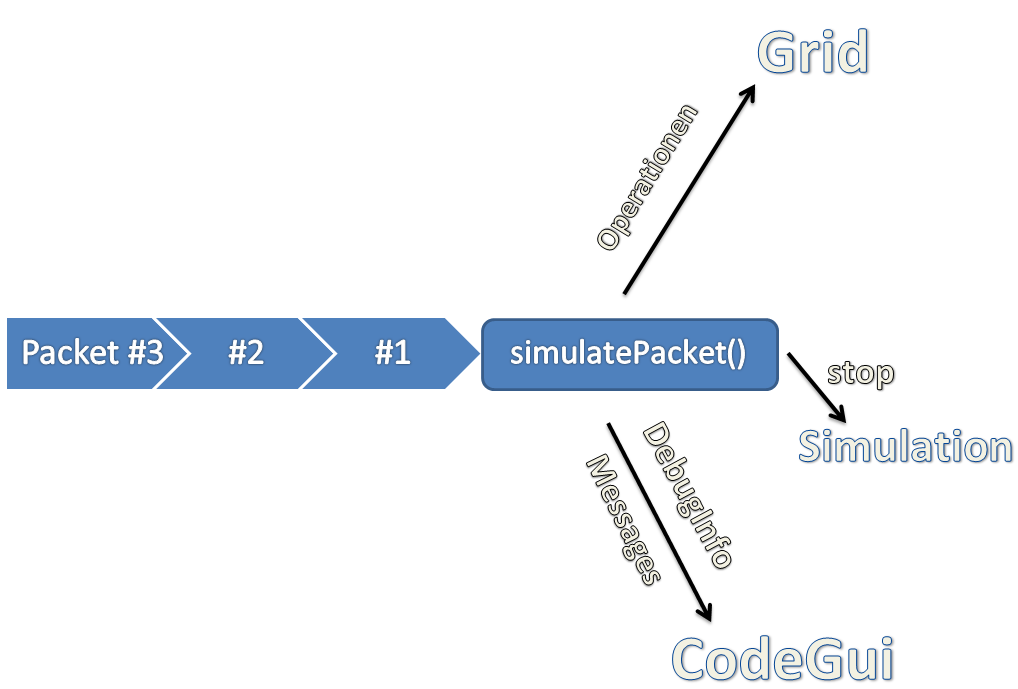
\includegraphics[scale=0.37]{client/socket-queue.PNG}
\end{frame}

\begin{frame}
\frametitle{CodeGUI}
\begin{center}
	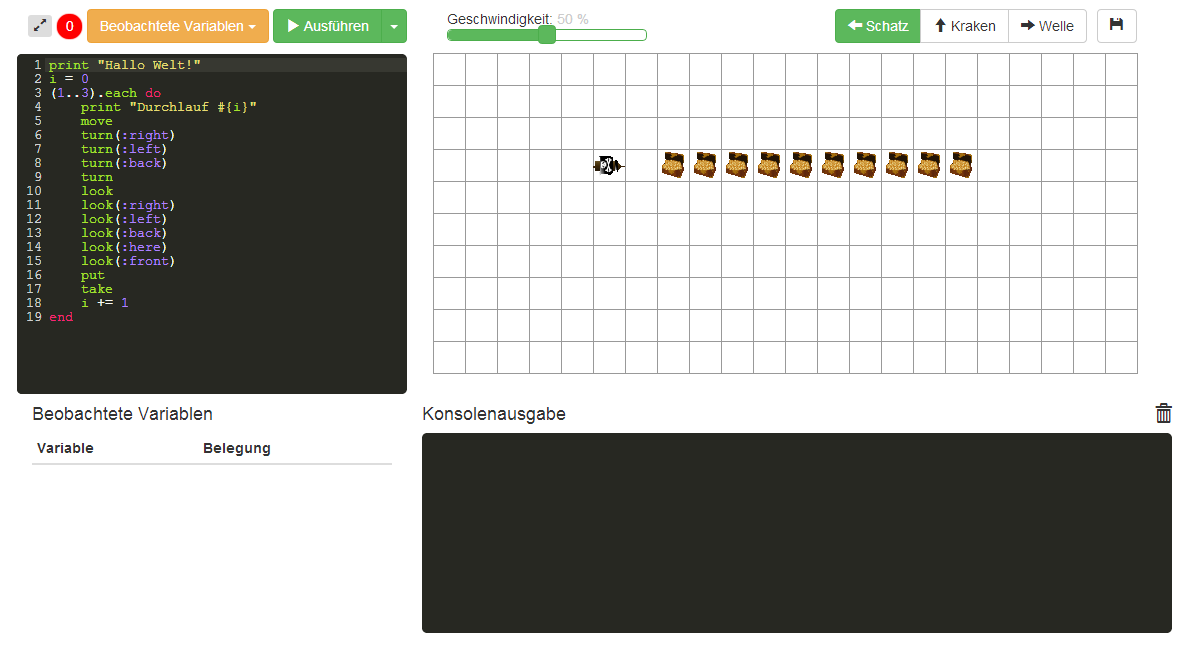
\includegraphics[scale=0.35]{client/client}
\end{center}
\end{frame}

\begin{frame}
\frametitle{Grid}
\begin{center}
	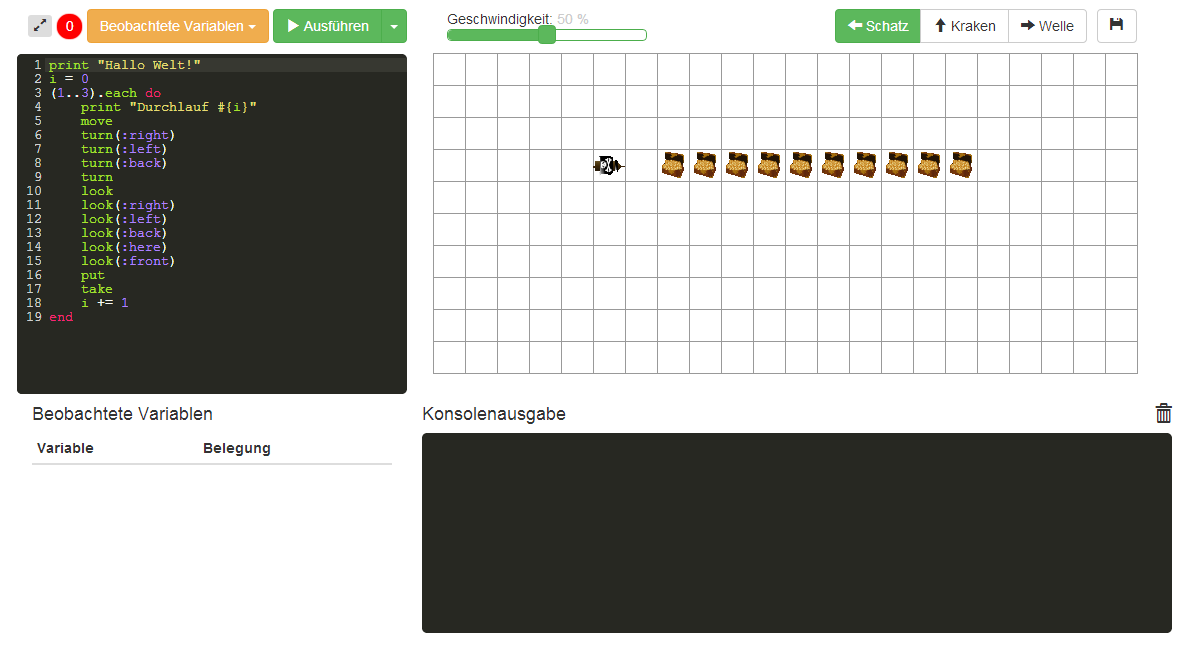
\includegraphics[scale=0.35]{client/client} %TODO
\end{center}
\end{frame}


\end{document}